\section{Objective}
In this experiment a Sagnac-interferometer is used in combination with a HeNe-laser is used to determine the refractive indices of glass and air. To achieve this the Interferometer is first adjustet and the visibility measured to guarantee a high quality in the interference pattern.
\section{Theory}
\label{sec:Theorie}
intererometry uses the effect of interference between lightwaves to make measurements for example regarding properties of certain materials like in this case the refractive indices of glass and air. To achieve interference several factors have to be taken into consideration, which will be discussed in the following chapter.
\subsection{Coherence}
When trying to observe interference between lightwaves it is important to consider, that interference occurs only with coherent light. This means, the different lightwaves have to have a constant phase relationship with each other to make interference possible. This property of light is called coherence and is distinguished between spatial and temporal coherence. Real lightsources emitt light in a certain spectrum and therefore constantly shift their phase, which means that a constant phase relation can only be achieved within a certain timeframe. Perfect monochromatic light theoretically is perfectly temporally coherent but can not be achieved in reality. Spatial coherence is achieved when wavefronts do not shift their phase difference due to spatial differences between the propagating wavefronts. An example of spatially incoherent light is given in the case of two unparallel wavefronts. 

Coherence is a phenomenon that exists on a certain scale, meaning that light can not only be incoherent or perfectly coherent. This is quantified by the Degree of coherence:
\begin{equation}
 \tilde{\gamma}_{12}(\tau)=\frac{\bigl<\tilde{E}_1(t+\tau)\tilde{E}^*_2(t)\bigr>_T}{\sqrt{\bigl<|\tilde{E}_1|^2\bigr>\bigl<|\tilde{E}_2|^2\bigr>}}
\end{equation}
with the electric fields $E_1$, $E_2$ and the relative offset $\tau$. The degree of coherence takes up values between $1$ and $0$ with $\gamma_{12}=1$ indicating perfect coherence.
\subsection{Polarisation}
Another important factor in interference of transversal waves like lightwaves is the polarisation of the wave. This describes the orientation of the plane in which the electric filed oscillates. The most important distinction in terms of polarisation is between linear and circluar/elliptical polarisation where the electric field vector is not polarised in a single plane but rotates. Linearly polarised light can be described by the polarization angle and generated from unpolarized light by using a polarisation filter, which only allows the component with the corresponding polarization angle to pass. Linearly polarized lightbeams can only produce interference if they have the same polarization angle. 
\begin{figure}
\centering
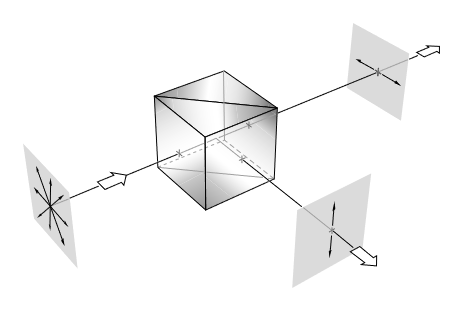
\includegraphics[width=0.6\textwidth]{PBSC}
\caption{Depictioin of a Polarising beam-splitter cube splitting unpolarised light into the s-polarised and p-polarised components. \cite{Hecht_2018}}
\label{fig:PBSC}
\end{figure}
A polarizing beam-splitter cube (PBSC) can be used to split light with a certain polarization into two perpendicular components. The transmitted beam is then polarized parallel (p-polarization) and the reflected beam perpendicular (s-polarization) to the incident plane. The effect of a PBSC on unpolarized light is depicted in Figure \ref{fig:PBSC}.
\subsection{Visibility}
A metric to describe the quality of an interference pattern is the so called visibility:
\begin{equation}
V=\frac{I_{max}-I_{min}}{I_{max}+I_{min}}
\end{equation}
which quantifies the contrast between the minimum Intensity $I_{min}$ and maximum Intensity $I_{max}$. The intensity is proportional to the square of the electric field strength $I\propto E^2$. 

More precisely the intensity of two interfering lightbeams can be described as:
\begin{equation*}
I \propto \bigl<|E_1\cos(wt)+E_2\cos(wt+\delta)|^2\bigr>
\end{equation*}
Assuming a phase difference of $\delta_{max}=n2\pi$ for complete constructive interference at the maximum and $\delta_{min}=(2n+1)\pi$ with $n\epsilon N^0$ for destructive interference at the minimum and consequently using $\cos(wt+\delta_{max})=\cos(wt)$ and $\cos(wt+\delta_{min})=-\cos(wt)$ the corresponding intensities can be calculated:
\begin{gather*}
I_{max/min}\propto \bigl<\cos^2(wt)(E_1\pm E_2)^2\bigr> \\
\iff I_{max/min}\propto E_1^2\pm 2E_1E_2 + E_2^2 
\end{gather*}
The strengths of the electric fields $E_1$ and $E_2$ is determined by the polarisation angle $\Phi$ of the initial light beam with the electric field strength $E_0$ before beeing split by the beam-splitter cube:
\begin{equation*}
\begin{pmatrix} E_1 \\ E_2\end{pmatrix}=E_0\begin{pmatrix}\cos(\Phi) \\ \sin(\Phi)\end{pmatrix}
\end{equation*}
Inserting this into the previous equation yields:
\begin{equation}
I_{max/min} \propto E_0^2(1\pm 2\sin(\Phi)\cos(\Phi))
\end{equation}
When inserting the results for the Intensities into the visibility it can be expressed depending only on the polarization Angle:
\begin{equation}
V (\Phi)=2\sin(\Phi)\cos(\Phi)
\end{equation}
\subsection{Refractive indicex of glass}
Using a glass holder holding two glass plates placed in the interferometer the refractive index of the glass can be determined based on the number of observed maxima or minima:
\begin{equation*}
M=\frac{\Delta \phi}{2\pi}
\end{equation*}
with the phase shift $\Delta \phi$ depending on the rotation angle of the glass plate $\Theta$ and the refractive index of the glass $n_{glass}$:
\begin{equation}
\Delta \phi=\frac{2\pi}{\lambda_{vac}}D\bigl( \frac{n_{glass}-1}{2n_{glass}}\Theta^2+O(\Theta^4)\bigr)
\end{equation}
With the vacuum-wavelength of light $\lambda_{vac}$ and the thickness of the glass plate $D$. Because the plates in the glass holder are already rotated by an angle of $\pm10°$ the formula for the phase shift has to be slightly changed and results in a linear relationship between the number of Maxima and the rotation angle:
\begin{gather}
M=\frac{D}{\lambda_{vac}}\frac{n_{glass}-1}{2n_{glass}}((\Theta+10°)^2-(\Theta-10°)^2)=\frac{D}{\lambda_{vac}}\frac{n_{glass}-1}{n_{glass}}2\Theta*10° \\
\iff n=\frac{1}{1-\frac{M\lambda_{vac}}{D2\Theta*10°}}
\end{gather}
\subsection{Refractive index of air}
The refractive index of air can be determined analogously by placing a gas cell of Length $L$ in the beam. This again results in a phase shift of
\begin{equation*}
\Delta \Phi=\frac{2\pi}{\lambda_{vac}}(n_{air}-1)L
\end{equation*}
corresponding to a refractive index of:
\begin{equation}
n_{air}=\frac{M\lambda_{vac}}{L}+1
\end{equation}
Alternatively the Refractive index of air can also be determined using the Lorentz-Lorentz-Law:
\begin{equation}
\frac{n_{air}^2-1}{n_{air}^2+1}=\frac{Ap}{RT}
\end{equation}
which describes the relationship between refractive index, pressure $p$ and temparature $T$. In this case $A$ denotes the molrefraction value and $R$ the universal gas constant.
\cite{sample}
